\section{Introduction}

\begin{frame}{Writing Secure Java Code}
	As one of the most widely used languages on the planet, a lot of security critical code is written in Java.
	
	Developers of applications that may interact with sensitive information must take steps to ensure the \textit{confidentiality} of that information is maintained. They can do this by:
	
	\begin{itemize}
		\item Following the Oracle Secure Coding Guidelines
		\item Running their application with a \texttt{SecurityManager} installed
		\item Following the Principle of Least Privilege
	\end{itemize}
	
	What they usually can't do is \textit{prove it}.
\end{frame}

\begin{frame}{Secure Applications: Why IF}
	content...
\end{frame}



\begin{frame}{Java is Vulnerable}
	\begin{columns}
		\column{0.55\textwidth}
			37 vulnerabilities in the JRE were recorded in the US National Vulnerability Database in 2016.\newline
			
			13 were listed as `critical', with a CVSS score $ > $ 9.0, indicating complete compromise of Confidentiality and Integrity \cite{nvd:jdk2016cvss9}.\newline
			
			This is in the \textit{JRE alone}, without considering the thousands of Java libraries and applications in existence.
		\column{0.45\textwidth}
		\begin{figure}
			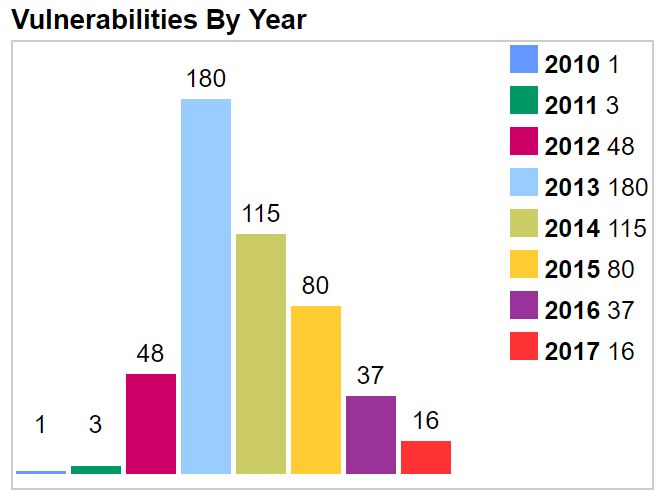
\includegraphics[scale=0.25]{content/images/cvedetails_vulnsperyear.png}
			\caption{Total CVEs by year \cite{cvedetails:jdk2016}}
		\end{figure}
	\end{columns}	
\end{frame}



\begin{frame}{Thesis Topic}
	One avenue for providing \textit{provable} Confidentiality to programs is applying \textit{Information Flow} policies, leading to the question:
	
	\begin{block}{Key Thesis Question}
		Can Information Flow be used to provide practical improvements to the Confidentiality of Java programs?
	\end{block}
	
	To answer this question, this thesis aims to evaluate both the relevance of information flow-based security, and current implementations of it, to determine:
	
	\begin{enumerate}
		\item What practical security benefits Information Flow can provide
		\item Whether Information Flow is viable for real world applications
	\end{enumerate}
\end{frame}